\documentclass[ 12 pt]{article}
\title{g12 note correction procedure}
\date{\today}
\usepackage{graphicx}
\usepackage[a4paper]{geometry}
\usepackage{microtype}
\renewcommand{\rmdefault}{ptm}  
\usepackage{lipsum}
\usepackage[english]{babel}
\setlength{\parindent}{0.2in}
\setlength{\parskip}{\baselineskip}
\usepackage{secdot}
\usepackage{amssymb}
\usepackage{amsmath}
%\usepackage[pdftex]{hyperref}
\usepackage{epsfig}
\usepackage{cancel}
\usepackage{verbatim} 
\usepackage{listings}
\usepackage{epstopdf}
\usepackage{color}
\usepackage{framed}
\usepackage[colorlinks=false, pdfborder={0 0 0}]{hyperref} 
\usepackage{cleveref}

 \begin{document}

\section{Correction question and g12 answer}
\begin{itemize}
\item \textbf{Tagger and RF calibration Figure 3 shows a jump in resolution. Why is that?}


This is due to the finalization of the production trigger, which requires higher energy photons. As also shown in Fig. 2, the high energy T-counters have better resolutions. With a trigger that requires the presence of a higher energy photon, the overall resolutions changes. However, the individual T-counter timing resolution remains the same. 

\item \textbf{Fig 12 shows good alignment of start counter for entire run period. However the resolution has steps. Any explanations why, for earlier runs, the resolution is a bit worse? Is there an understanding of this effect? How does this affect the data analysis? How does the start counter timing resolution compares to other run periods?}

The ST resolution was obtained by assuming a gaussian distribution, while in reality the ST-RF timign differences are not exactly gaussian. Therefore, it IS affected by background, beam current, trigger. The steps are about 30ps and 10ps respectively, and we use the best start counter hit in our event selection. Therefore, we do not expect any significant effect.

\item \textbf{ST efficiency. How did you determine this number? Is it for any particle of any momentum at any angle? Have you looked at the efficiency for protons and pions separately? Have you looked at the efficiency for different paddles?
For instance infamous paddle 9 has known problems with efficiency and resolution. How is this efficiency used in the analysis?}\\
The efficiency of the start counter was calculated by examining the number of tracks with a ST hit after track reconstruction. The ST fired 91.6\% of the time, this was calculated from run 57000 since it is a good run and included in production data.\\ We do not account for the bad resolution of paddle 9 specifically. The effect should be absorbed by the track-dependent inefficiency corrections. 

\item \textbf{DC calibrations. Has the DC alignment with B=0 data been done? Show the results.}

Yes, the alignment was done using $B=0$ data. The note (section 2.5) has been updated accordingly.

\item \textbf{DC efficiencies. Show a comparison of the real data and MC data with DC efficiency map applied.}

The DC wire efficiencies were computed for each wire using the whole data set, using the CLAS utility PDU. An example of this is shown in the beginning of DC calibration section. Simulation data all use the GPP to apply this efficiency map. This is standard practice in CLAS. The data compares very well with simulation. 

\item \textbf{There is nothing in the note about CC calibration and efficiency. It is also not clear if CC timing is used in the analysis or not.}

This has been addressed now in the note in Section 2.6.1. Also, the CC timing is not used in standard g12 analysis.


\item \textbf{EC calibration and efficiency. You don't say anything about energy calibration 
and energy response. You have quite a few dead strips. They not only affect 
efficiency but also affect energy response. How did you handle this? What 
procedures (corrections) were used to reconstruct photon energy and pi0 
2gamma decay?}\\


The EC energy calibration quality can be demonstrated by the two photon invariant mass ($\pi^0$) as a function of run number (Fig. 35 in section 2.8). The mean is very close to the expected value. The knock-out of bad and inefficient EC strip are summarized in Table 18. 

\item \textbf{Target thickness. You quote target length uncertainty of 0.2 cm. Please 
explain where is this number coming from. Have you accounted for the 
thermal contraction of the cell? At the end, for normalization purposes, you 
need the number of target protons. Just put this number with all corrections 
applied. This is the single number everybody should use for this dataset.}

Point taken. We do not quote a separate systematic uncertainty associated only with target length.


\item \textbf{For yield and PID stability check, and evaluation of the related systematic 
uncertainty, show the average number of protons and pion per event on a
run-by-run basis. The pull distributions of these quantities can be used to 
estimate the associated systematic uncertainty.}

The average number of protons and pions on a run-by-run basis was monitored during the storage, and we did not observe any significant instability. Furthermore, we believe this is already shown in the omega yield plot in section 4.3. The uncertainty associated with this effect is estimated to be around $0.5~\%$. 

\item \textbf{For the photon flux systematic uncertainty, evaluate two sources.\\
Comparison of different normalization runs.
Pull distribution of normalized yield.}

sections 4.2 and 4.3. plots address this, just need to add a number to the text (sys unc) ????

\item \textbf{Describe the procedure for photon flux binning to arbitrary bin size.}

Done! (Details in Sec 4). 


\item \textbf{When you compare yields with different beam current you apply a multiple 
photon correction. There may be different ways of doing it. Explain the 
procedure.}

For this particular study, only one photon was chosen (randomly) if there is multiple photons in the chosen time bucket. If the probability of having two photons is (ignoring more than two photons) P, the normalized yields is corrected by a factor of $\frac{1}{1-0.5P}$. indeed dependent on the beam current, and is corrected accordingly.

\item \textbf{When you discuss the photon energy correction, you say that the tagger 
magnetic field is not measured. This is not correct. We had a Hall probe in the 
tagger magnet and it was read in EPICS together with magnet current.}

It has been corrected accordingly in the note. 

\item  \textbf{Fig. 57 caption says beam current, but shows beam energy.}

It was a typo and has been corrected.

\item \textbf{Fig. 51 is confusing. What is JTG PCor? Yellow points show the best match to 
neutron mass, but if the legend is correct the momentum correction is not 
applied. Please, clearly explain what exact procedure must be used for 
momentum/energy corrections.}

The g12 momentum correction was derived by Johann, hence the name of JTG. Fig. 51 was indeed confusing, and it has  now been replaced (at a different location), to demonstrate the effect of all g12 corrections being applied together (End of Section 3.3, Fig. 68). 

\item \textbf{In addition to missing mass distributions, show some invariant mass 
distributions. They are independent of photon energy and will show if the 
momentum corrections are good regardless of photon energy correction.}

The invariant mass of $K^+\pi^0$, showing the $K^{*+}$, and the $K^+K^-$ invariant mass showing the $\phi(1020)$,  have been added in the note (chapter 6). The mass of $K^0$ reconstructed from $\pi^+\pi^-$ pairs can also be seen to be where it is expected (Fig. ~58).  All known narrow states in g12 have been shown to be within $1$~MeV of the PDG values.

\item \textbf{Reference for [eloss] is CLAS Note 2007-016 }

It has been corrected.

\item \textbf{You refer to the g9 momentum correction. In general the procedure may be
applied to g12 data. However direct comparison does not make sense since
the configuration of the experiments were very different.}

We do not use g9 momentum correction. And the note has been modified accordingly.


\item  \textbf{The lepton id is based on the analysis of the EC and CC information, however 
no discussion of the CC calibration is included in chapter 2.}

The is related to the previously addressed issue. 


\item  \textbf{The CC cuts used in the present analysis includes a cut on Npe and a cut on 
the CC hit angle that is related to the track direction. No cut on the time 
correlation between CC hit and, for example, TOF hit associated to the same 
track is used: this is a standard cut used in all recent electron beam analysis 
used to reject misidentified pion. Why is this not applied?}

Using the current cuts of NPE and hit angle, the suppression of di-leptons was sufficient without including additional cuts on the CC. This method of lepton PID, involving di-leptons, was established during the g7 run period. Further g12 analyses that involve single lepton PID could include this as a cut.



\item \textbf{The EC cuts used in this analysis are based on the total energy deposited in
the calorimeter, E\_calo, and exploit the fact that E\_calo/p is almost a constant
for leptons. This is a typical selection criteria used in most electron run
analyses: usually the way this selection is illustrated is by plotting E\_calo vs p
and displaying the cuts on this graph. We suggest replacing figures 69-75
with these simple plots: this would make easier for a reader, familiar with
lepton analysis, to understand the selection cuts}


???


\item \textbf{The note refers to the g7 lepton id scheme in explaining the chosen cuts: in
g7 however, not only cuts on the total calorimeter energy but also cuts on the
inner and outer energy were used: why were these not considered necessary
in the present analysis?}

IsLepton() in g12 was made to be a balanced between good
lepton selection without being aggressively restrictive.  Like any other
PID, it is up to the individual analyses to show the validity of their
particle selection, and make additional cuts as needed.



\item \textbf{In chapter 2.7.1, the knockout of bad EC strips is explained in details. We
assume the loss of efficiency due to the strip knockout was accounted for by
applying the same knockout function to both real data and mc data (used for
the efficiency evaluation). Can you please confirm this is what was done (the
explanation in the note is not very clear about this point)? The strip knockout
will induce a worsening of the calorimeter energy resolution that becomes
dependent on the sector and on the track impact point. How was this
accounted for?}

The bad strips are knocked out both in data and simulation. The effect of energy resolution worsening is not accounted. If this is an important issue for a particular analysis, it has to be investigated separately.

\item \textbf{Was the stability of the EC calibration checked as a function of run number
(for example monitoring the E\_calo/p ratio)?}

Not exactly. However, the $\pi^0$ mass was monitored as a function of run number and stable.


\item \textbf{To be able to judge the effectiveness of the lepton id cuts, we suggest
showing the CC photoelectron distribution for the initial and final lepton
sample: a typical hint of how clean the final sample is the disappearance of
the peak at about 2 photoelectrons which is visible in the initial plots.}

In our procedure, which is derived from the g7 group, a cut on the npe is part of the lepton ID. The effectiveness can be demonstrated in the figures in section 3.4. 




\item \textbf{You use the DC residual match to determine smearing parameters. Once this 
is done, show how the reconstructed momentum resolution compares with 
the one from simulation.}

While deriving the smearing parameters, we also monitored the TOF timing resolution as well as invariant mass resolutions such as $\phi(1020)$. The data compares very well with the data. For example, the overall TOF resolution is about $215$~ps in the simulation, very close to the data which is just above $200$~ps.

\begin{figure}[h!]\begin{center}
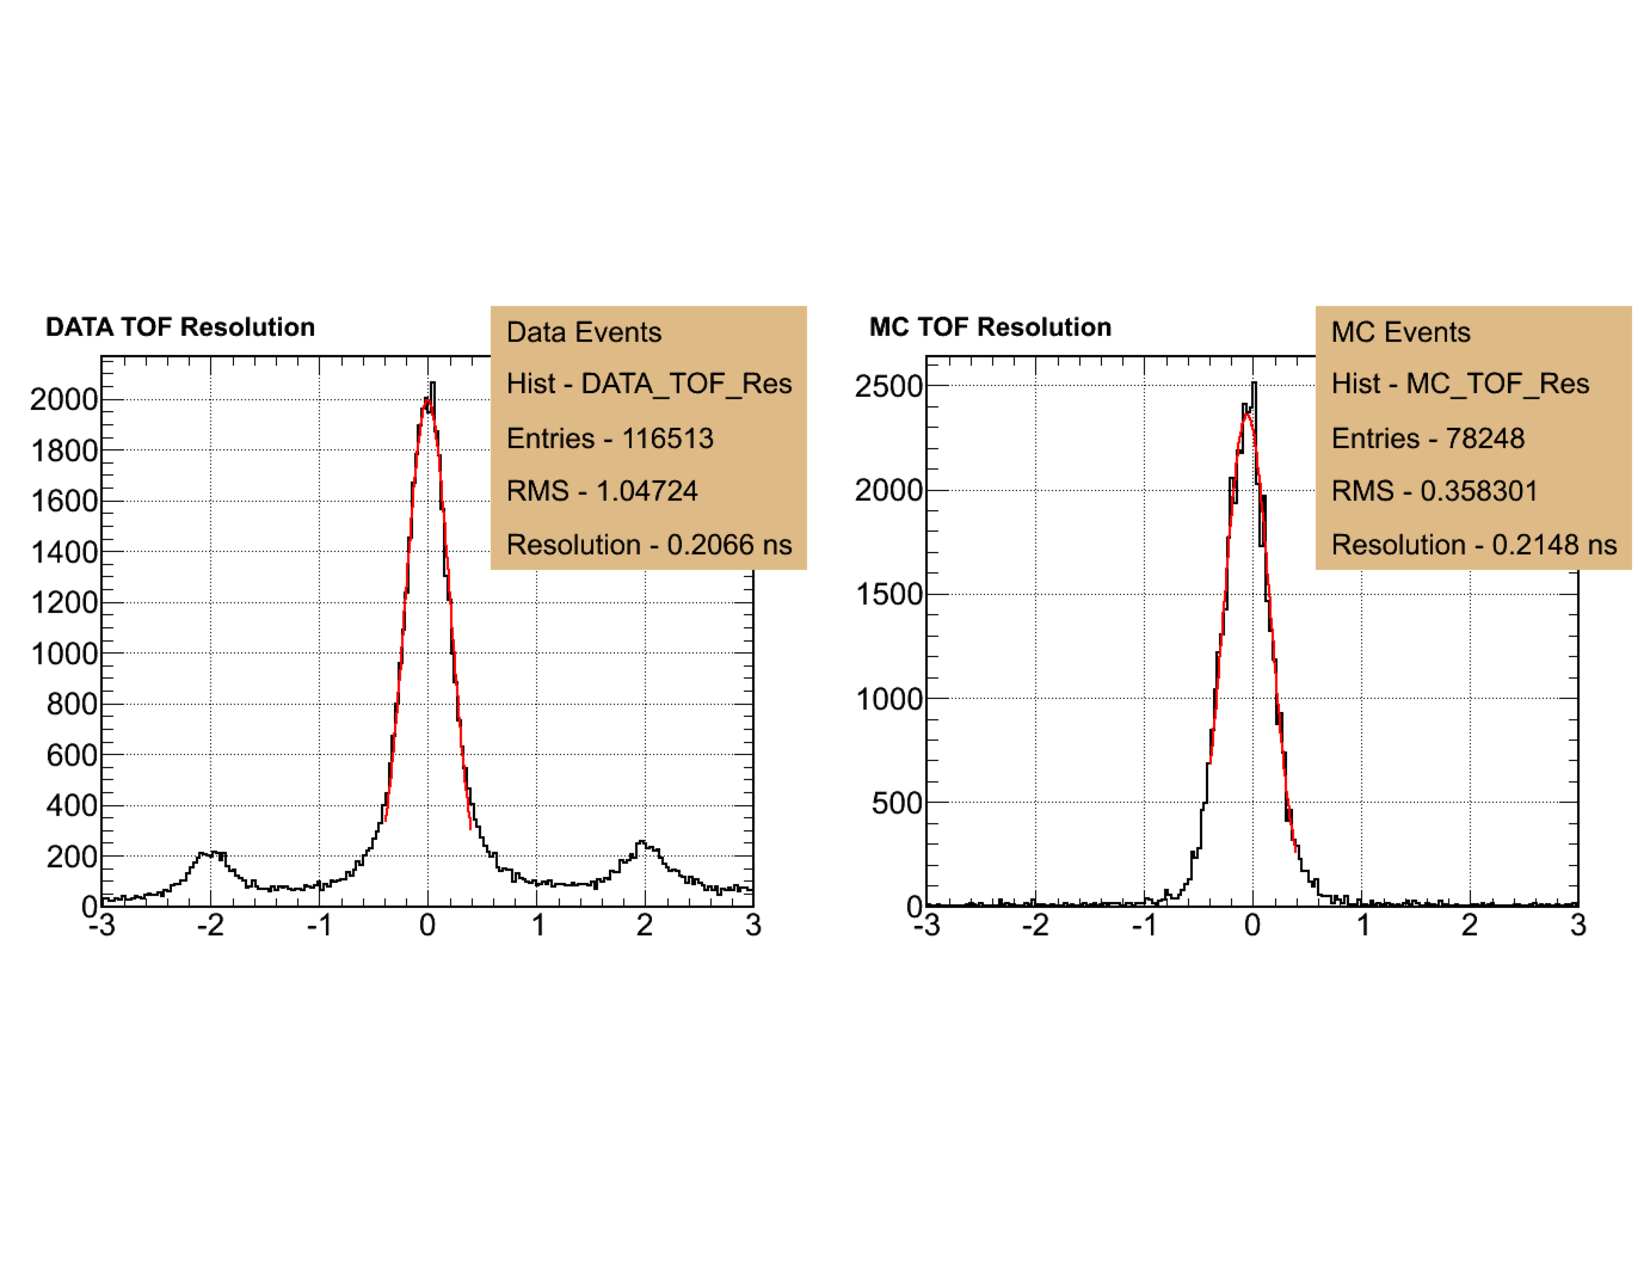
\includegraphics[width=12cm,height=8cm]{figures/calib/tof/TOF_gpp.pdf}
\caption[]{ TOF resolution for data (left) and simulation(right)}
\end{center}\end{figure}

\item \textbf{To demonstrate that efficiencies are accounted for correctly, show
comparisons of various distributions (angular, occupancies?) between data
and simulation.}
This has been done for g12 in many topologies. For illustration purpose, the momentum and angular distributions for $e^+$ are shown here, comparing data and simulation. 

\begin{figure}[htpb]\begin{center}
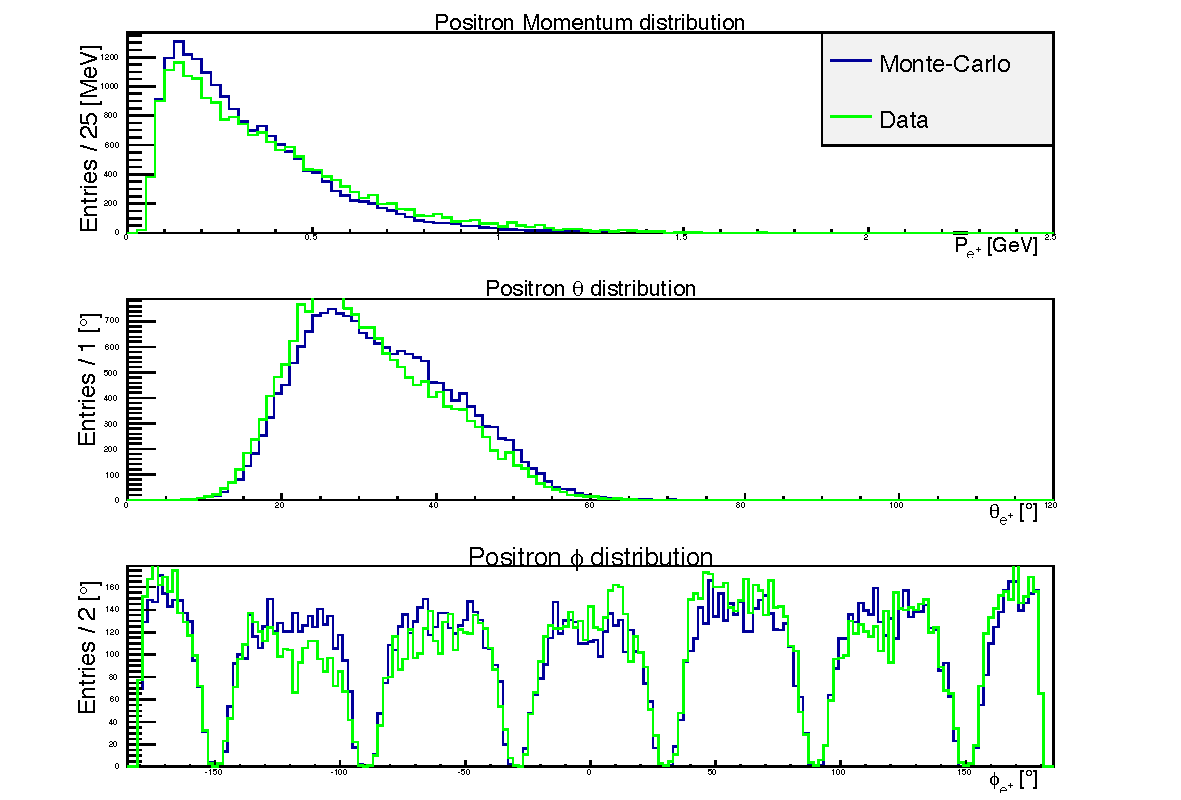
\includegraphics[width=16cm,height=8cm]{figures/calib/ec/Positron_Kinematics_new.pdf}
\caption[Positron Kinematics]{\label{fig:positronkinematics}Momentum and angular comparison of data to simulation for the positron.}
\end{center}\end{figure}


\item \textbf{Did you knock out bad tagger counters in the simulation?}

Two known bad energy regions in the tagger: (2.975,3.175) (dead/bad paddle) and (3.475,3.575). G12 group do not use events from these two regions.

\item \textbf{If input events for GSIM are in the form MCVX/MCTK banks, GSIM can 
properly generate the TAGR bank. Among other things it modifies photon 
energy and assigns it to the center of the Ebin. If you use the PART bank as an 
input to GSIM, your event generator is supposed to generate the TAGR bank.
How it is done in your event generator? Does it account for tagger sag?}\\

The TAGR bank was generated in the same manner in both cases. The tagger sag was accounted in the data during the cooking stage. For simulation, there is no tagger sag.


\item \textbf{Fiducial Region Selection: Were these determined from simulated events? 
Why not from real data?}

It is derived from real data.



\item \textbf{p.87 bottom: Why 50\%? How was this criterion chosen? Above 50\% the 
acceptance still varies as fast as below 50\% - is the acceptance in regions 
above 50\% better described by GSIM?}\\

 g12 has three sets of fiducial cuts (nominal, tight and loose), not just the 50\% (nominal) cuts. One should always try them all and used the difference to derive systematic uncertainties associated with the fiducial cuts. This of course, is applicable only when statistics of the specific topology allows.

\item \textbf{p.88: We would like to see all the phi distributions - can be given with a link
to a web site.}\\

Unfortunately we did not keep all the plots. Once the number were extracted after careful examination of those plots, we only kept the numbers and eventual software tools for applying the fiducial cuts. 


\item \textbf{Fig. 83: We would like to see these plots for all sectors. The point at 0.4 GeV/c 
has a very small uncertainty, while the two neighboring points have much 
larger uncertainties - is it understood why?}\\

This is really an artifact of statistics. Even if this point was taken out, the fit would still work.

\item \textbf{Provide the size of the different skims, how many events?}\\

total size:\\

211 TiB (exclusive)\\
31 TiB (additional)\\
26.2 Ge (Billion Events)\\
exclusive skims:\\
%\begin{table}
\begin{tabular}{ c c c }
size	     &      events	&     skim\\
50 TiB	 &    6.2 Ge	&    1-1ckaon1ctrk\\
31 TiB	 &    3.8 Ge	&    2-2pos1neg\_not\_1ckaon1ctrk \\
68 TiB	 &    8.4 Ge	&    3-2ctrk\_not\_2pos1neg\_1ckaon1ctrk \\
62 TiB	 &    7.7 Ge	&    4-not\_2ctrk\_2pos1neg\_1ckaon1ctrk \\
263 GiB &	32.6 Me &	   5-other
\end{tabular}
%\end{table}
\\
additional skims:\\
%\begin{table}
\begin{tabular}{ c c c }
size     &	events  &	skim\\
17 TiB &	2.1 Ge  &	6-1lepton\\
13 TiB &	1.6 Ge  &	7-4ctrk\\
1 TiB	& 124 Me & 	8-ppbar\\
\end{tabular}
%\end{table}

\item \textbf{What banks are included in the cooked files? Are the SEB and GPID banks 
included?}\\

here they are in alphabetical order:

CC CC01 CCPB CCRC CL01 DCPB DSTC EC EC1 EC1R ECHB ECPB ECPC ECPI ECS EPIC EVNT FBPM HBER HBID HBTR HEAD HEVT HLS LCPB MVRT PART RGLK S1ST SC SC1 SCPB SCR SCRC SCS ST1 STN0 STN1 STPB STR STSN SYNC TAGE TAGI TAGR TBER TBID TBTR TDPL TGBI TGPB TGS TRGS TRKS TRL1\\
SEB related banks (EVNT etc) are included. GPID is not.


\item \textbf{Non-physics events are included in in a separate skim. How can one 
synchronize them with physics events? They have different numbering 
sequences.}\\
Events can be coordinated by timestamp; Alternatively, one can always go back to the raw data if someone in the future find it useful to include these non-physics data.


\item \textbf{Yesterday we found out from Zulkaida's talk that some additional normalization correction of ~15\% has been applied to cross section. I don't think there is anything said about this correction in g12 note. Is this common correction to be applied to all cross sections? If so it has to be included in the note with explanation how it was obtained.}\\

That global correction is not technically correct, but it happens to be very close to what should be applied. G12 compares the reconstruction efficiency between real and mc data (ratio of the acceptances for each track). This leads to an overall correction about 5\% for each track, but it is slightly kinematical variable dependent. If someone is looking at 2-track events, then the correction would have been smaller. The g12 procedure for applying this track-dependent inefficiency correction has now been documented  (Section 6.1). It is important to point out that this correction naturally absorbs any detector/trigger inefficiency that was not fully accounted for in our procedures such as the GPP smearing.



{\it The following questions are still being worked on:}


\item \textbf{TOF efficiency and bad paddles. The selection of bad paddles is based on raw 
ADC and TDC information. This is only good for the initial selection. After 
that you should look at the PID quality of individual paddles. We know from 
other data sets that sometimes the occupancy looks good but particle ID is 
not good. The bad particle ID could be due to bad resolution or sometimes we 
see “double peaking” in which the timing is jumping between two different 
states. If it is stable within the run it is fixable by adjusting offsets run-by-run. 
However these instabilities appear even within a single file. It would be good 
to see timelines for vertex time difference and resolutions for protons and 
pions vs. run number for individual paddles.}\\

We have checked the timelines for the time of flight resolution for each paddle, using cooked events containing $p \pi^{+} \pi^{-}$ in the final state. For the $\pi^{+}$ and $\pi^{-}$, the difference between the measured time-of-flight and the expected time-of-flight for a given run was plotted and fitted to a Gaussian. This was done for every paddle and every run.  Most paddles were well calibrated and stable but a few paddles that had not been previously knocked out had drifts on either the resolution or the mean, or shows poor calibration. Table~\ref{tab:tofko.additional} shows which paddles should ideally be knocked out due to this. However, the track dependent efficiency correction was derived without these paddles being knocked out. Consequently, these paddles should not be knocked out if one uses the track dependent efficiency correction. If one would like to use these additional time-of-flight knockouts, then one would need to re-derive the track dependent efficiency corrections, which will be provided. Figure~\ref{plot:example.goodpaddle} shows an example of a (the vast majority of the ) good paddle's resolution and mean  while figure~\ref{plot:example.badpaddle} shows and example of a bad paddle. Combining the number of new bad paddles judging from the resolutions, and the occupancy of these paddles, we estimate that about 3\% of the data is impacted. However, this effect is already addressed by the existing track dependent efficiency correction. In fact, this 3\% effect is probably one of the main sources of the around 5\% correction needed in that correction.  In addition, a few paddles in sector 5 demonstrated a shift in resolution of about 100 ps for about 1.5\% of the runs. Figure~\ref{plot:example.badsector5} shows an example of this. Ideally, these should be recalibrated and recooked, but this solution is unrealistic, and the impact so small since it is only 8 paddles having 100 ps drift for 10 runs out of more than 650 runs (less than 0.1\%) . 

\begin{table}
\begin{minipage}{\textwidth}
\begin{center}
\begin{singlespacing}

\caption{\label{tab:tofko.additional}Additional paddles to knock out due to drifts in the mean $\Delta$ TOF or resolutions}

\begin{tabular}{lc}

\hline \hline

Sector 1: & 25, 26\\
Sector 2: & 18, 25, 27\\
Sector 3: & 1, 18, 32\\
Sector 4: & 8, 19 \\
Sector 6: & 24 \\

\hline \hline

\end{tabular}

\end{singlespacing}
\end{center}
\end{minipage}
\end{table}


\begin{figure}\begin{center}
      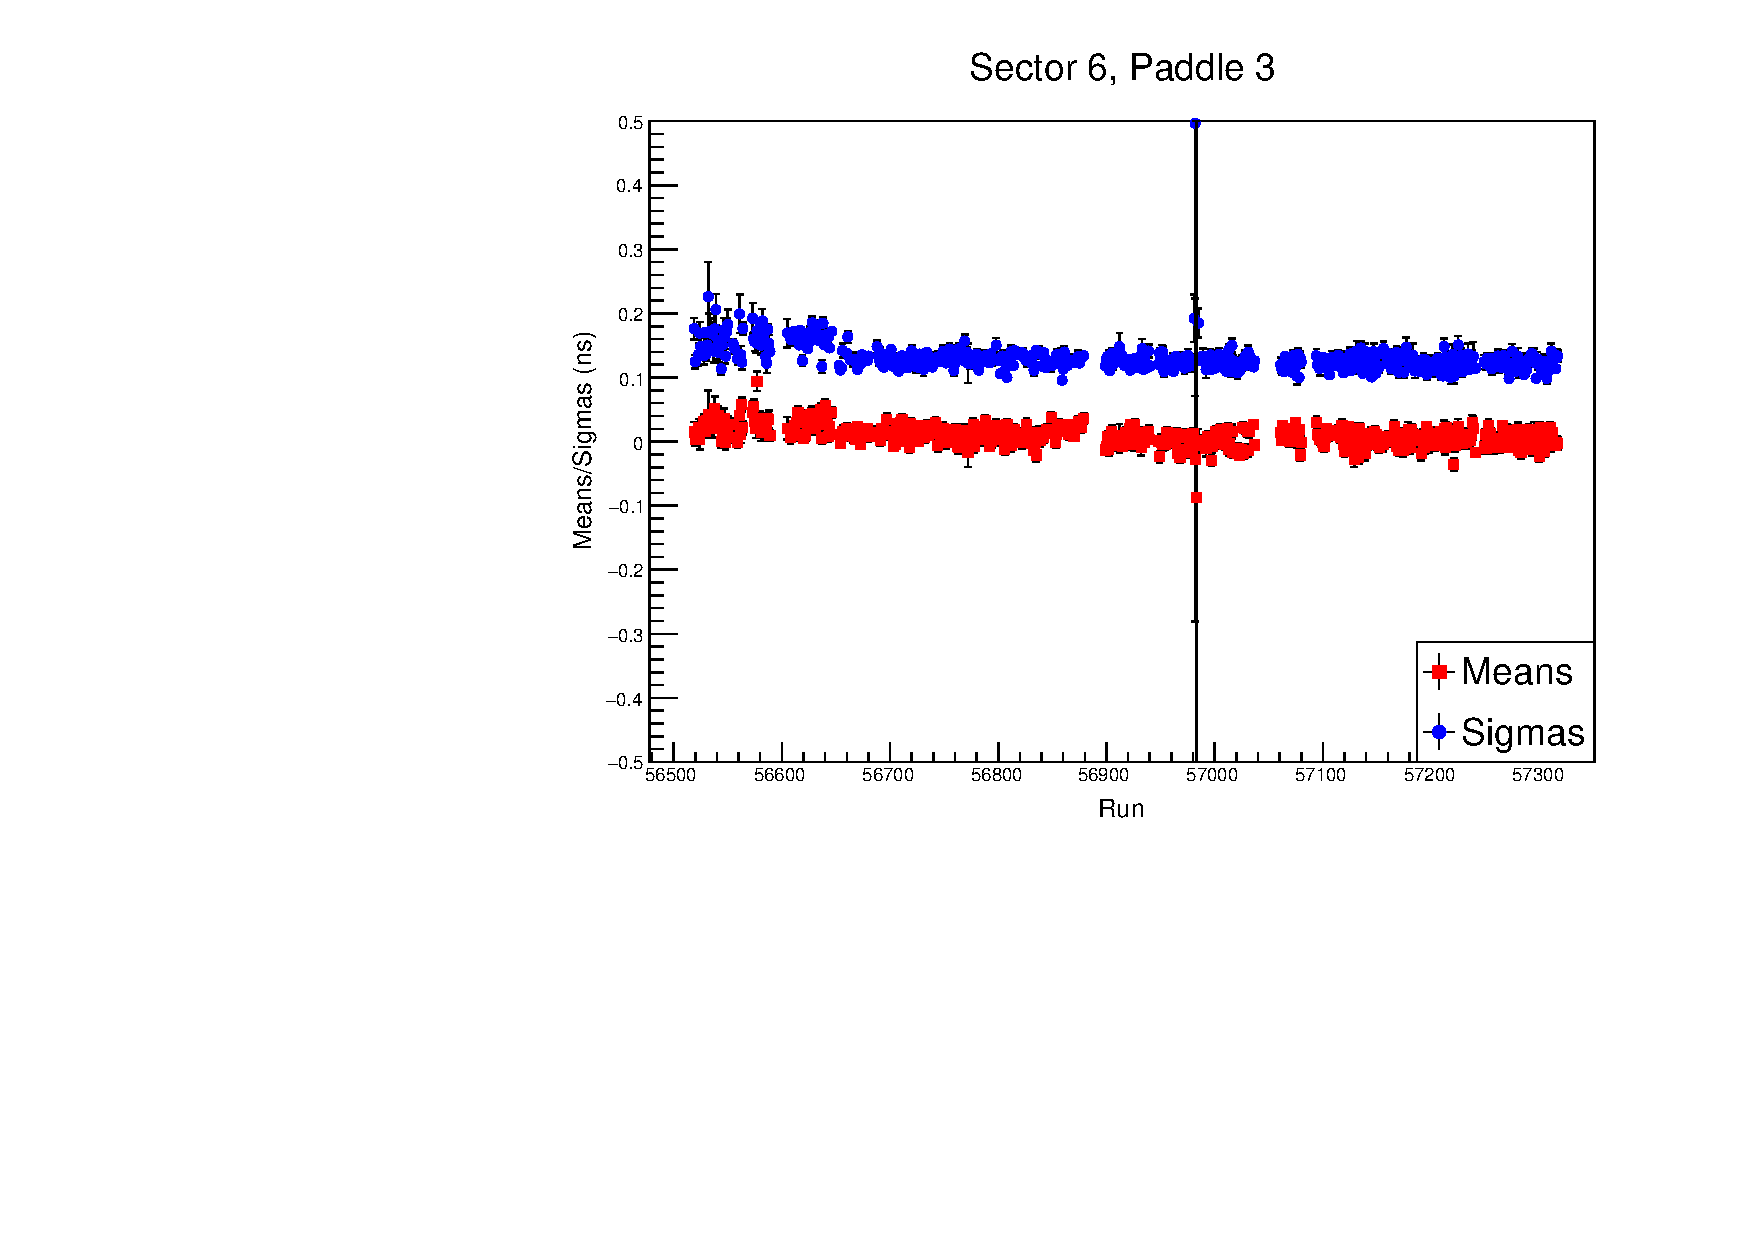
\includegraphics[width=0.6\columnwidth]{figures/calib/tof/goodexample.pdf}
   \caption{\label{plot:example.goodpaddle}TOF resolution as a function of run number for a good paddle}
\end{center}\end{figure}

\begin{figure}\begin{center}
      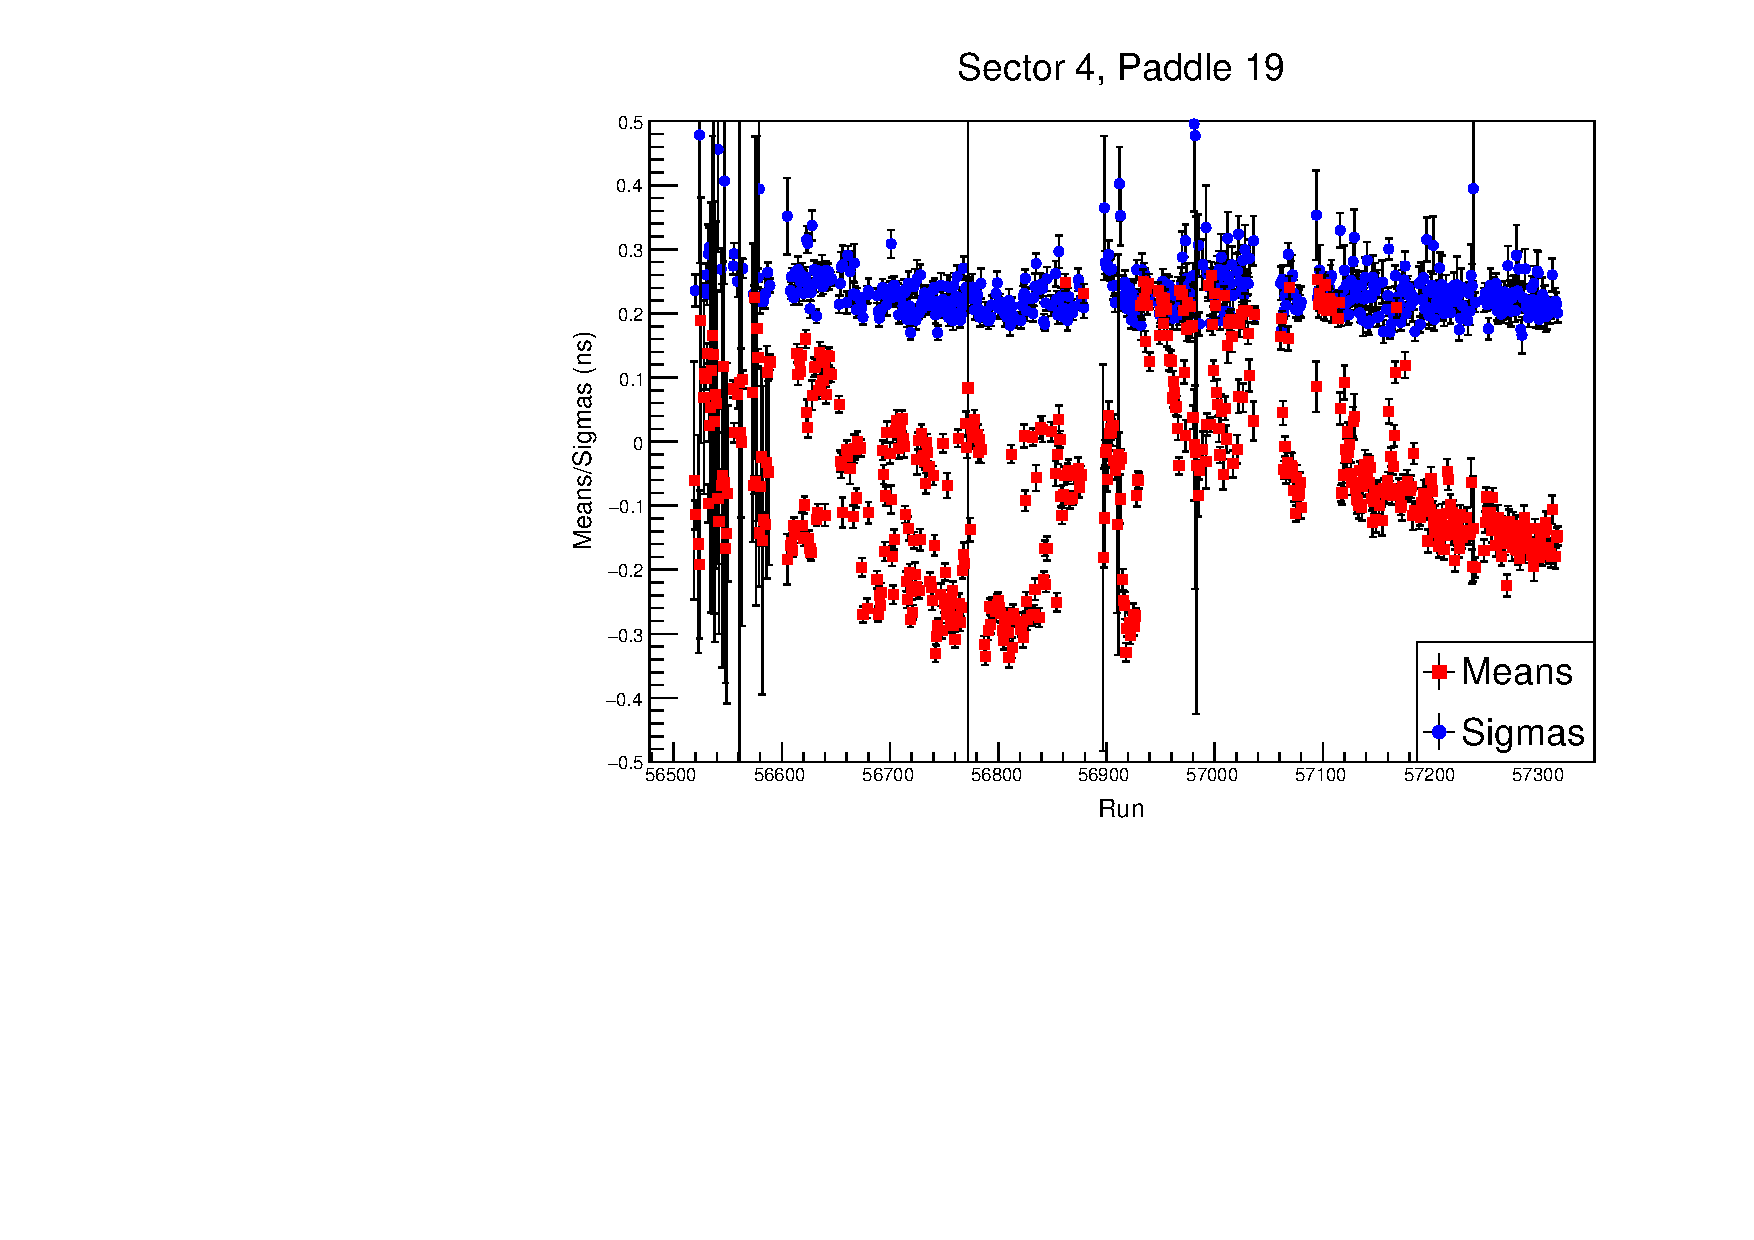
\includegraphics[width=0.6\columnwidth]{figures/calib/tof/badexample.pdf}
   \caption{\label{plot:example.badpaddle}TOF resolution as a function of run number for a bad paddle}
\end{center}\end{figure}

\begin{figure}\begin{center}
 	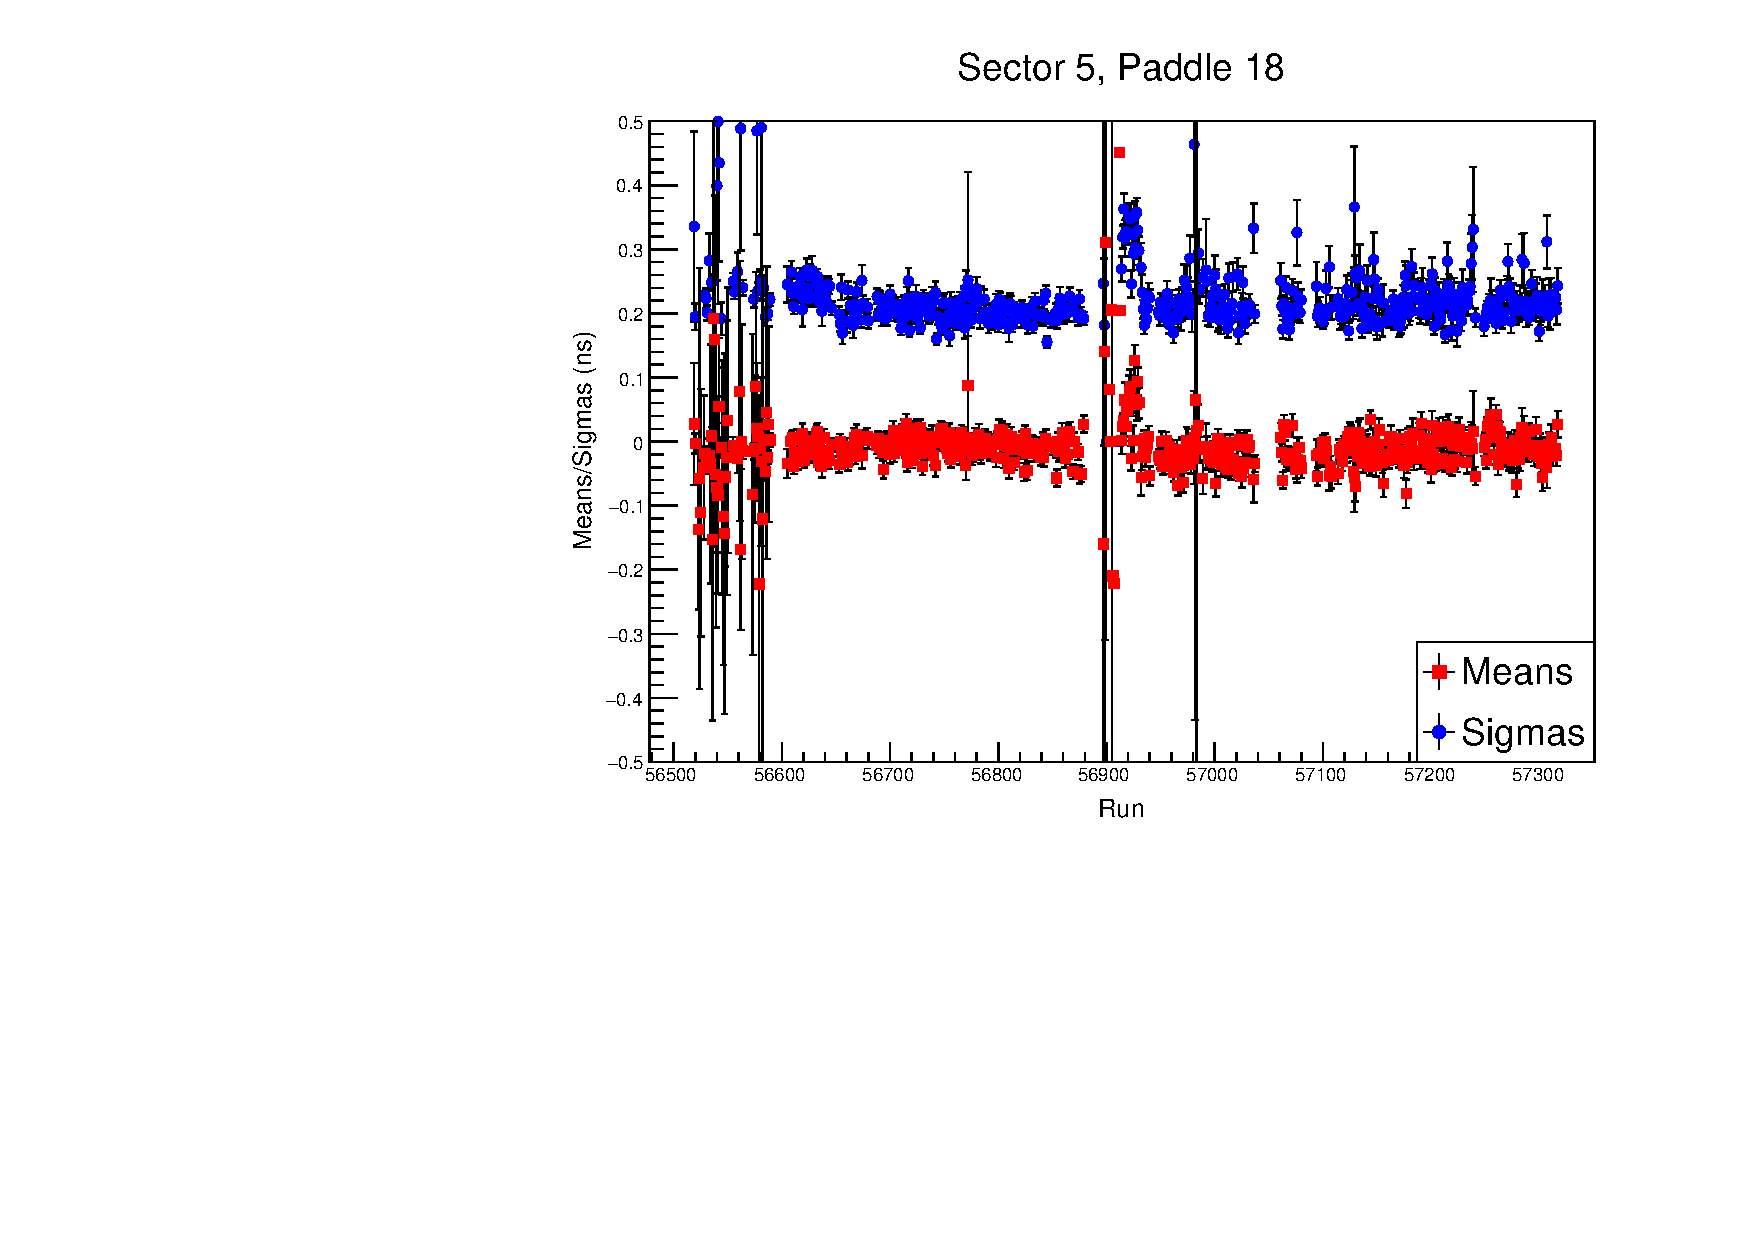
\includegraphics[width=0.6\columnwidth]{figures/calib/tof/badsector5.pdf}
   \caption{\label{plot:example.badsector5}A few sector 5 paddles' resolutions shift for a few middle runs}
\end{center}\end{figure}


\item \textbf{TOF uses different discriminators with different thresholds for TDCs and for
trigger. It was discovered by the g13 group that some of the counters are
inefficient in the trigger but look fine in TDC. What has been done to address
this trigger inefficiency?}

%Being worked on by Rafael. We should be able to show that the resolutions are stable. However, we do not plan to knock out additional paddles, because the track dependent inefficiency correction absorbed this effect. If we were to do a new knockout scheme, everything would have to be changed again and there is nothing concrete we could gain from it.

See previous answer.


\item \textbf{When you compare cross sections to previous measurements please 
compare in the same kinematical bins. A strong forward peak pushes other 
point to the axis and it is not possible to judge if they agree or not. In addition 
to overlaying two data sets, show their ratio. Even without it we see that in 
some bins the agreement is not very good. Make something similar to pull 
distributions as well, to see if there is a bias.}\\

Being done by Zulkaida/MK/Johann.


\item \textbf{Beam polarization. While you well describe the study performed to verify
helicity assignment, you don?t provide an exact recipe for the user on how to
obtain the sign of the helicity. Was it direct or delayed reporting of helicity?
Should the user include the half-wave plate state or it was already accounted
for? Ideally would be good to have a function which takes care of all this and
returns the sign of helicity for a given event. The degree of the photon
polarization then will have to be calculated for the ?good? photon using
electron beam polarization and polarization transfer. This can be made a
standard function which will pull out electron beam polarization for a given
run. This will make life easier for those who will analyze this data in the
future. Eq. 11 is not correct - need to explain how the photon polarization
was implemented so that the yield asymmetry is converted into a
polarization observable (event by event, integrated over all events, else?);
level of agreement between g12 and g1c control asymmetries must be
quantified; Was Icirc monitored per run? Why do you not reproduce exactly
the same Icirc as in [17] and visualize/quantify the level of agreement for
exactly the same energy bin. We agree that this method is good to determine
the overall sign of the helicity assignment, however there still may be a
polarization bias, which is not determinable from this comparison, due to the
acceptance effect on the extracted Icirc.}



Statistical errors for the polarization of the beam is shown on table 20 in the note. The total systematic error is estimated to be 5\%.

There is a method, to be stored as \begin{verbatim} /work/clas/clasg12/clasg12/clas6-trunk/include/gethelicity.h \end{verbatim}, 
that takes care of the issue on how to obtain the helicity with the proper sign and plainly returns it.


%FIU and FSU independently measured the beam-helicity asymmetry and were in good agreement with each other. The pull distribution between FIU and FSU is shown in figure~\ref{fig:pol:g12compare} and the pull distribution between FIU and g1c's results are shown in figure~\ref{fig:pol:g12g1ccompare}. Both FIU and FSU use approximately 15\% of the entire dataset (due to the independence of the two measurements, their selection of the data is most likely not the same). Figure~\ref{fig:pol:g12g1ccompare} shows good agreement between g12 and g1c's beam-helicity measurement.

Eq. 11 had a typo and was corrected. The correct equation is 
\begin{equation}
I_\odot = \frac{1}{P_{\gamma}} \frac{N^{+} - N^{-}}{N^{+} + N^{-}}
\end{equation}

We investigated the systematic uncertainty of the asymmetry measurements by comparing the g12 two pion beam helicity results and g1c results, as well as two independent g12 analyses (FIU by Rafael and FSU by Zulkaida. Fig.~\ref{fig:pol:g12compare}). The pull distribution between the g12 (only using 15\% of the statistics)  and g1c results (Fig.~\ref{fig:pol:g12g1ccompare}) does not show major shift between the two experiments. Furthermore, the two independent analyses (FIU and FSU) are self consistent. And the 0.01 shift between the g12 and g1c results are consistent with an expected $\sim 3\%$ overall polarization uncertainty measurement.  Using the half of the mean from the g12/g1c pull distribution, and divide it by the maximum of around 0.18 for the asymmetry measurement, we conclude that the overall asymmetry measurements and related polarization observables should be around 3.3\%. It is important to point out that these asymmetry measurements are performed at different angular bins, while the two experiments, having different set up and acceptance, does not have exactly the same angular distributions. So the current comparison is only sufficient to address the overall uncertainty or shift. The exact bin-by-bin comparison would be addressed in a more systematic manner once all g12 statistics are used.

\begin{figure}[htpb]
\begin{center}
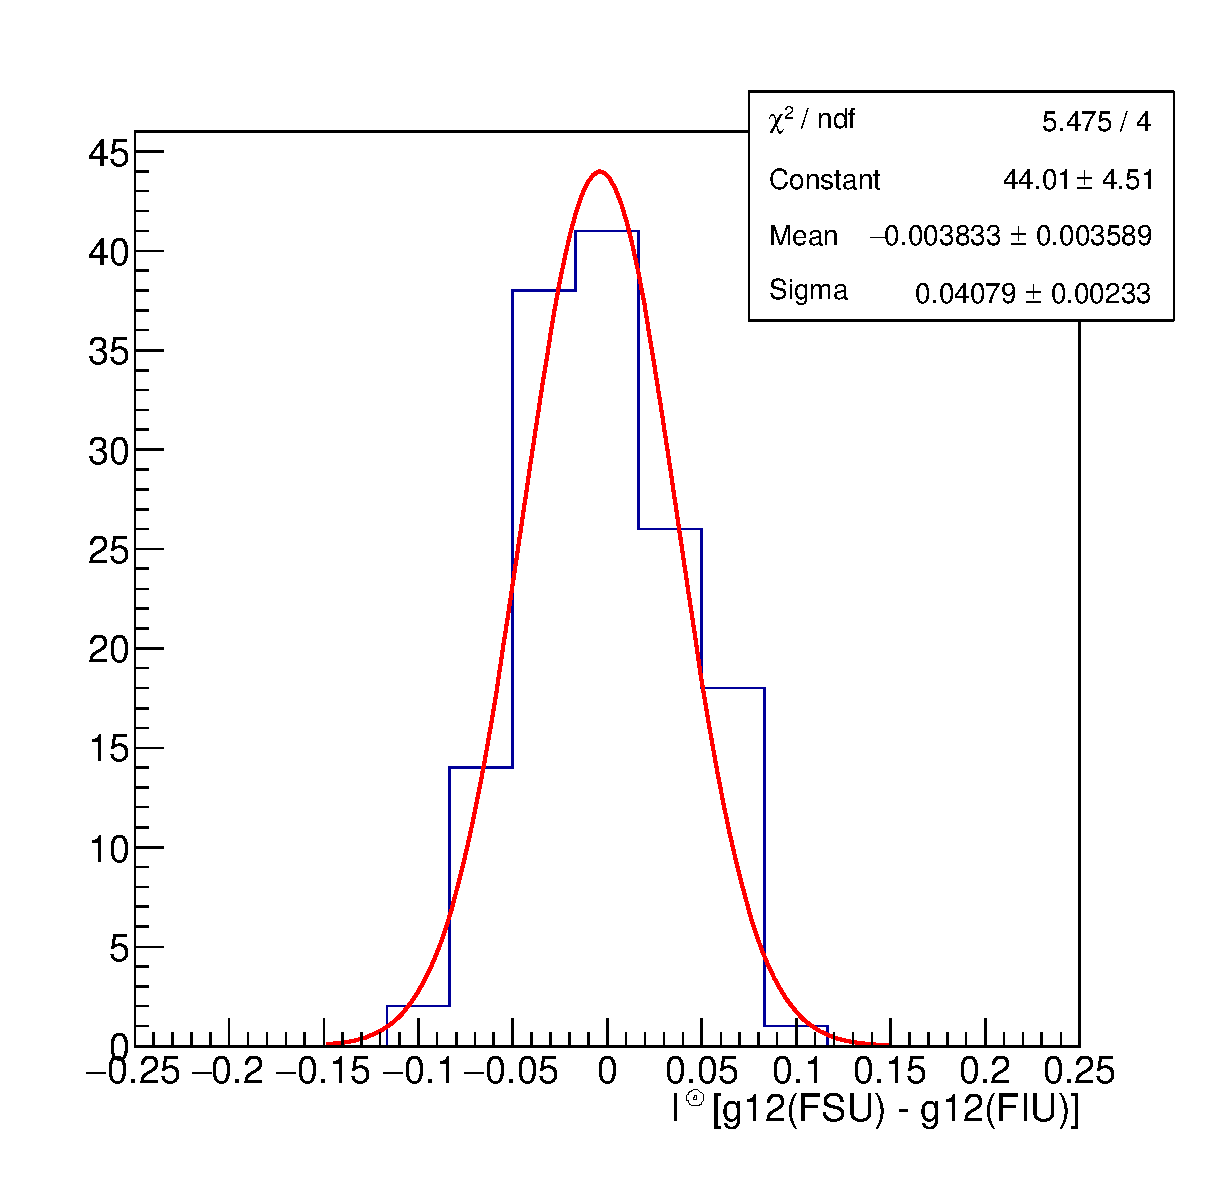
\includegraphics[width=0.6\columnwidth]{{figures/calib/pol/g12compare}.eps}
\caption{\label{fig:pol:g12compare} Pull distribution between FIU and FSU $I^{\odot}$ }
\end{center}
\end{figure}

\begin{figure}[htpb]
\begin{center}
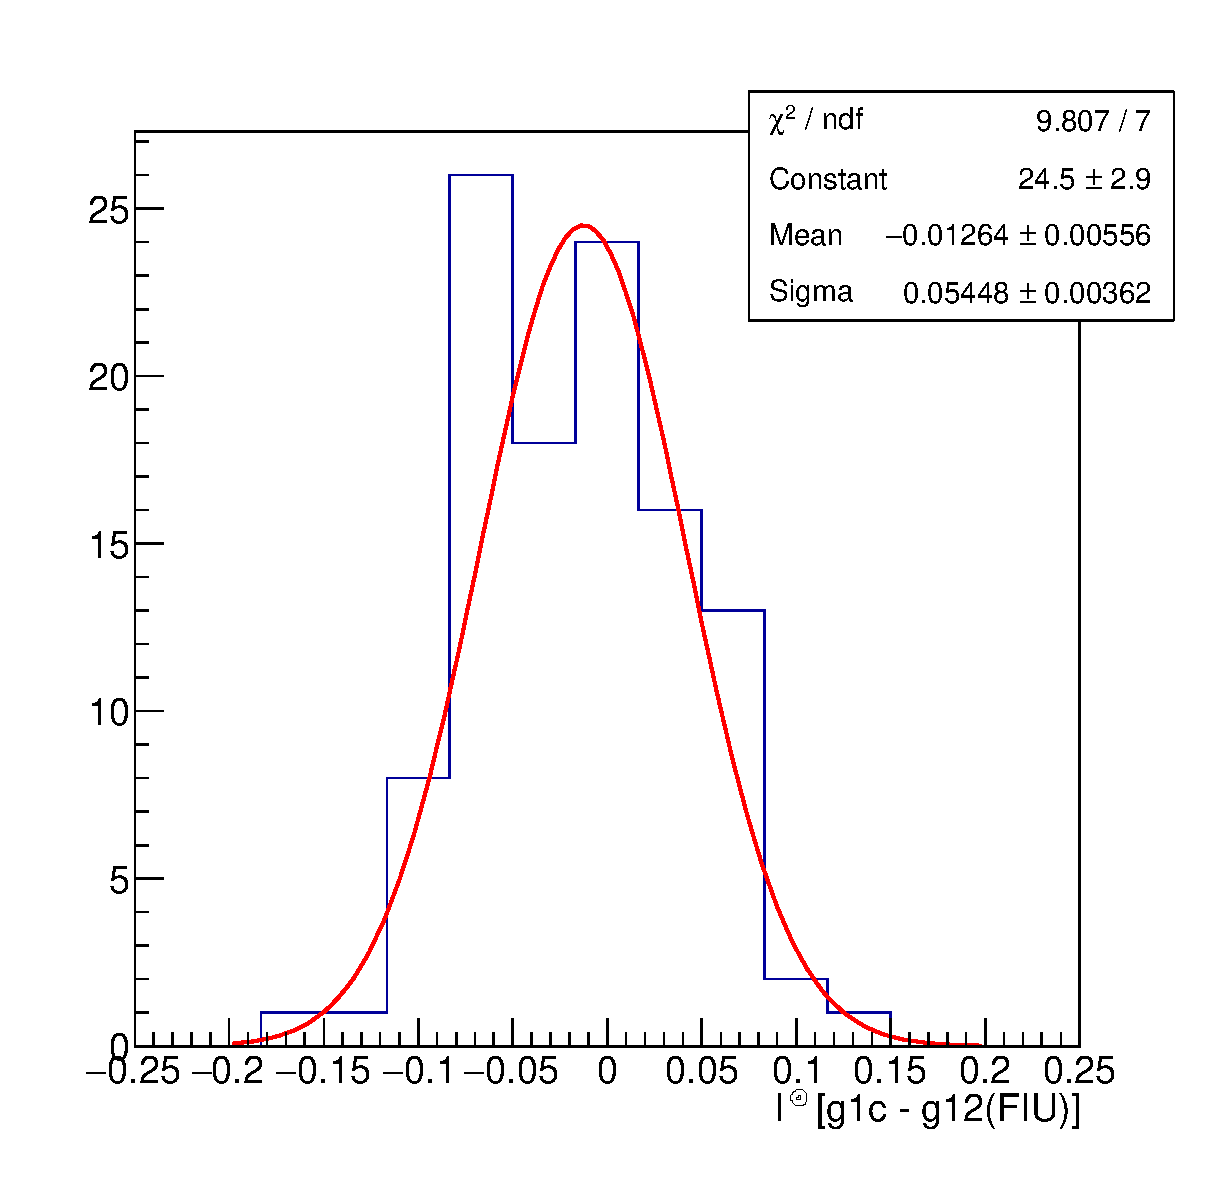
\includegraphics[width=0.6\columnwidth]{{figures/calib/pol/g12g1ccompare}.eps}
\caption{\label{fig:pol:g12g1ccompare} Pull distribution between g12 (FIU) and g1c $I^{\odot}$ }
\end{center}
\end{figure}

\end{itemize}






















\end{document}